% Provenance (never printed): cycle 4 SVT, "La planete Terre": sedimentation,
% from sediment to sedimentary rock, fossilisation, fossils and layers as a
% record of past environments; see sources/book1/PROVENANCE.md. Book 1,
% grade 7, chapter 4.
% Vocabulary guard: first chapter allowed to use "sediment"; the principles of
% relative dating (superposition, fossil succession and the rest) and "unconformity" are
% g7.5's and are not named here; fossils as evidence of evolution are the
% biology books' (one sentence of prose).
\chapter{Sedimentos y fósiles}\label{ch:g7:sediments-and-fossils}

El Gran Cañón, en Arizona (Estados Unidos), tiene de media \qty{1.6}{km}
de profundidad. Sus paredes están hechas de capas de \omterm{def:g3:stones-pebbles-sand:rock}{roca}, unas encima de
otras, rojas, marrones, grises y de color crema. En la capa más alta, la
caliza de Kaibab, los guardas del parque señalan conchas: las conchas de
braquiópodos, animales que vivían en el fondo de un \omterm{def:g2:water-on-earth:ocean}{mar}. Esa \omterm{def:g3:stones-pebbles-sand:rock}{roca} se formó
en el fondo de un \omterm{def:g2:water-on-earth:ocean}{océano}, y hoy forma el borde del cañón, muy por encima
del \omterm{def:g4:world-physical-map:altitude}{nivel del mar}.
% ledger: nps:grca-depth, nps:grca-fossils, nps:grca-kaibab

\begin{omfigure}
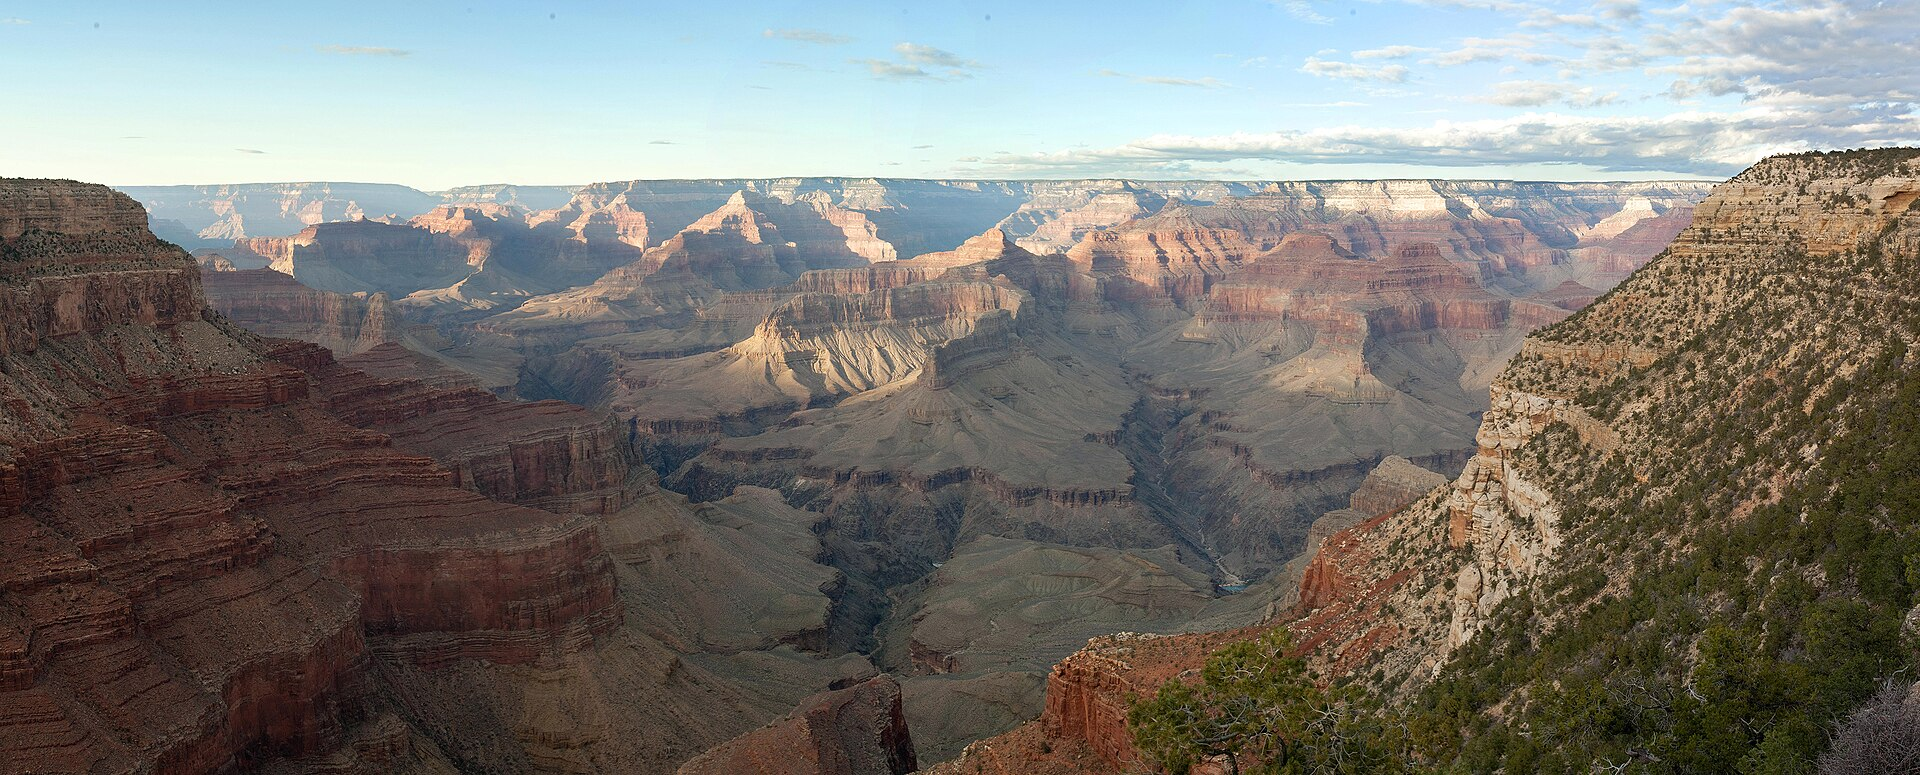
\includegraphics[width=\linewidth]{images/book1/g7-grand-canyon.jpg}

{\small El Gran Cañón visto desde Hermits Rest, en su borde sur: capa tras
capa de \omterm{def:g3:stones-pebbles-sand:rock}{roca}, desde el borde hasta el fondo. Fotografía del NPS, por
Kristen M. Caldon (dominio público, vía Wikimedia Commons).}
% ledger: commons:grand-canyon
\label{fig:g7:sediments-and-fossils:canyon}
\end{omfigure}

¿Cómo se convierte un montón de \omterm{def:g3:stones-pebbles-sand:sand}{arena} y \omterm{def:g3:stones-pebbles-sand:sand}{barro} sueltos en \omterm{def:g3:stones-pebbles-sand:rock}{roca} sólida?
¿Cómo puede una concha durar tanto tiempo que acaba dentro de un
acantilado? ¿Y qué nos dicen las capas y los \omterm{def:g7:sediments-and-fossils:fossil}{fósiles} sobre cómo eran los
lugares hace mucho tiempo?

\begin{recall}
Las \omterm{def:g3:stones-pebbles-sand:rock}{rocas} se rompen lentamente en pedazos en la superficie
(\emph{\omterm{def:g5:water-shapes-the-land:weathering}{meteorización}}); el agua, el viento y el hielo se llevan los
pedazos (\emph{\omterm{def:g5:water-shapes-the-land:erosion}{erosión}}) y los depositan donde frenan y se detienen
(\emph{\omterm{def:g5:water-shapes-the-land:deposition}{sedimentación}}): primero los más pesados, y el \omterm{def:g3:stones-pebbles-sand:sand}{barro} fino solo donde
el agua está casi quieta (\cref{ch:g5:water-shapes-the-land}). Una
\emph{\omterm{def:g6:rocks-and-minerals:rock-families}{roca sedimentaria}} se forma en la superficie a partir de granos de
\omterm{def:g3:stones-pebbles-sand:sand}{arena} y de \omterm{def:g3:stones-pebbles-sand:sand}{barro}, o de conchas, depositados en capas y endurecidos:
arenisca, lutita, caliza. El \omterm{def:g6:rocks-and-minerals:rock-cycle}{ciclo de las rocas} transforma lentamente las
\omterm{def:g3:stones-pebbles-sand:rock}{rocas} de cada familia en las de las otras (\cref{ch:g6:rocks-and-minerals}).
\end{recall}

\section{Los sedimentos se depositan en capas}

Allí donde el agua, el viento o el hielo sueltan lo que llevaban, se va
formando un depósito suelto: \omterm{def:g3:stones-pebbles-sand:pebble}{grava} y \omterm{def:g3:stones-pebbles-sand:sand}{arena} en el lecho de un \omterm{def:g1:landscapes-around-us:water}{río}, \omterm{def:g3:stones-pebbles-sand:sand}{barro} en
el fondo de un \omterm{def:g1:landscapes-around-us:water}{lago}, \omterm{def:g3:stones-pebbles-sand:sand}{arena} en una playa o en una duna, conchas en el fondo
del \omterm{def:g2:water-on-earth:ocean}{mar}.

\begin{definition}[Sedimento]\label{def:g7:sediments-and-fossils:sediment}
Un \emph{sedimento}\index{sedimento} es un material suelto depositado por
el agua, el viento o el hielo: \omterm{def:g3:stones-pebbles-sand:pebble}{grava}, \omterm{def:g3:stones-pebbles-sand:sand}{arena}, \omterm{def:g3:stones-pebbles-sand:sand}{barro}, o las conchas y los
esqueletos de seres vivos. Se acumula en el fondo de los \omterm{def:g1:landscapes-around-us:water}{ríos}, de los
\omterm{def:g1:landscapes-around-us:water}{lagos} y de los \omterm{def:g2:water-on-earth:ocean}{mares}, y en tierra firme, donde lo sueltan el viento o el
hielo.
\end{definition}

Los \omterm{def:g7:sediments-and-fossils:sediment}{sedimentos} se depositan en un orden determinado. Cuando el agua
cargada de \omterm{def:g3:stones-pebbles-sand:sand}{barro} frena, los granos más grandes y pesados se hunden primero,
y los más pequeños y ligeros, al final. Cada vez que el agua cambia --- una
\omterm{def:g5:water-shapes-the-land:flood}{crecida} que trae \omterm{def:g3:stones-pebbles-sand:sand}{arena}, y después semanas tranquilas en las que solo llega
\omterm{def:g3:stones-pebbles-sand:sand}{barro} fino al fondo ---, los granos que se depositan también cambian, y
empieza una capa nueva. Poco a poco, el fondo de un \omterm{def:g1:landscapes-around-us:water}{lago} o de un \omterm{def:g2:water-on-earth:ocean}{mar} se
cubre de un montón de capas, con las más antiguas en la base del montón.
% ledger: usgs:strata, usgs:sediments-to-rock

\begin{omfigure}
\begin{tikzpicture}[font=\small, x=1cm, y=1cm]
  % land and river
  \fill[omLithAlluv] (0,3.0) -- (2.0,2.45) -- (2.0,0) -- (0,0) -- cycle;
  \fill[blue!35] (0,3.05) -- (2.0,2.5) -- (2.0,2.4) -- (0,2.95) -- cycle;
  % lake water
  \fill[omSea!45] (2.0,2.5) -- (12.4,2.5) -- (12.4,1.12) -- (3.0,1.2) -- cycle;
  \draw[blue!50!black, line width=0.6pt] (2.0,2.5) -- (12.4,2.5);
  % layers on the bottom: thick near the mouth, thinner far out
  \foreach \k/\c in {0/omLithSand, 1/omLithShale, 2/omLithSand, 3/omLithShale} {
    \pgfmathsetmacro{\yb}{0.2+0.25*\k}
    \pgfmathsetmacro{\yt}{0.2+0.25*(\k+1)}
    \fill[\c] (3.0,\yb) -- (12.4,\yb) -- (12.4,\yt-0.08) -- (3.0,\yt) -- cycle;
  }
  \draw[black!60, line width=0.3pt] (3.0,1.2) -- (12.4,1.12);
  \fill[omLithAlluv!80!black] (2.0,0) rectangle (12.4,0.2);
  \fill[omLithAlluv] (2.0,0.2) -- (3.0,0.2) -- (3.0,1.2) -- (2.0,2.45) -- cycle;
  % settling grains: big ones near the mouth, fine ones far out
  \foreach \x/\y in {3.3/2.1, 3.6/1.75, 3.9/2.25, 4.2/1.55, 3.5/1.35, 4.5/2.0} {
    \fill[brown!70!black] (\x,\y) circle (0.07);
    \draw[-{Stealth[length=1.3mm]}, black!60] (\x,\y-0.1) -- (\x,\y-0.32);
  }
  \foreach \x/\y in {6.5/2.2, 7.4/1.8, 8.3/2.15, 9.1/1.6, 9.9/2.05, 10.8/1.75, 11.6/2.1, 7.9/1.35, 10.4/1.3} {
    \fill[brown!50!black] (\x,\y) circle (0.025);
    \draw[-{Stealth[length=1mm]}, black!40] (\x,\y-0.05) -- (\x,\y-0.2);
  }
  \node[anchor=south, align=center] at (1.0,3.1) {un río en crecida\\[-2pt]trae arena y barro};
  \node[anchor=south, align=center] at (4.1,2.55) {la arena se deposita\\[-2pt]primero, cerca de\\[-2pt]la desembocadura};
  \node[anchor=south, align=center] at (9.2,2.55) {el barro fino se deposita despacio,\\[-2pt]lejos, donde el agua está tranquila};
  \draw[decorate, decoration={brace, amplitude=4pt}] (12.55,1.15) -- (12.55,0.2)
    node[midway, anchor=west, xshift=4pt, align=left, font=\footnotesize] {capas del\\[-2pt]fondo: arena,\\[-2pt]barro, arena, barro};
\end{tikzpicture}

{\small \omterm{def:g7:sediments-and-fossils:sediment}{Sedimentos} que se depositan en un \omterm{def:g1:landscapes-around-us:water}{lago} (un dibujo, no a escala).
Después de cada \omterm{def:g5:water-shapes-the-land:flood}{crecida} se deposita una capa de \omterm{def:g3:stones-pebbles-sand:sand}{arena}, y luego \omterm{def:g3:stones-pebbles-sand:sand}{barro} fino
en las semanas tranquilas que siguen: capa tras capa, el fondo se va
cubriendo.}
% ledger: usgs:strata
\label{fig:g7:sediments-and-fossils:lake}
\end{omfigure}

\begin{definition}[Capa sedimentaria]\label{def:g7:sediments-and-fossils:layer}
Una \emph{capa sedimentaria}\index{capa sedimentaria}, o
\emph{estrato}\index{estrato} (en plural, \emph{estratos}), es una lámina
de \omterm{def:g7:sediments-and-fossils:sediment}{sedimento}, o de la \omterm{def:g3:stones-pebbles-sand:rock}{roca} en que se ha convertido, depositada de una sola
vez. Tiene una base y un techo, y se distingue de las capas de encima y de
debajo por el tamaño de sus granos o por aquello de lo que está hecha.
\end{definition}

Los \omterm{def:g7:sediments-and-fossils:sediment}{sedimentos} se depositan a partir del agua o del aire, así que quedan
horizontales, como las páginas de un libro apoyado sobre una mesa. Cuando
se encuentran capas inclinadas o plegadas, es que algo las movió después
de formarse. La estratificación es la marca más clara de una \omterm{def:g6:rocks-and-minerals:rock-families}{roca
sedimentaria}: la has visto en las paredes del Gran Cañón.
% ledger: usgs:strata, nps:grca-kaibab

\begin{inthelab}[Capas en un tarro (en clase, con el profesor)]
Pon un puñado de \omterm{def:g3:stones-pebbles-sand:pebble}{grava}, dos puñados de \omterm{def:g3:stones-pebbles-sand:sand}{arena} y unas cucharadas de tierra
en un tarro de cristal alto; llénalo de agua, ciérralo bien y agítalo.
Déjalo en la mesa y observa durante unos minutos: la \omterm{def:g3:stones-pebbles-sand:pebble}{grava} llega al fondo
enseguida, la \omterm{def:g3:stones-pebbles-sand:sand}{arena} un poco después, y el \omterm{def:g3:stones-pebbles-sand:sand}{barro} fino mantiene el agua
turbia durante horas. Al día siguiente, añade un poco más de tierra y de
\omterm{def:g3:stones-pebbles-sand:sand}{arena}, agita suavemente y deja que se deposite otra vez. ¿Cuántas capas
puedes contar? ¿Qué granos hay en la base de cada una?
\end{inthelab}

\section{Del sedimento a la roca}

Una capa no se queda mucho tiempo en lo alto. Otras capas se depositan
encima, y después otras, y queda enterrada cada vez más hondo. Bajo el
peso de las capas de encima, los granos se aprietan unos contra otros y el
agua que había entre ellos es expulsada. El agua que se filtra a través
del montón deja \omterm{def:g6:rocks-and-minerals:mineral}{minerales} entre los granos, un cemento natural que los
pega. Con mucho tiempo, a medida que se acumulan más capas y se producen
lentos cambios químicos, el \omterm{def:g7:sediments-and-fossils:sediment}{sedimento} suelto de la base del montón se
convierte en \omterm{def:g3:stones-pebbles-sand:rock}{roca}.
% ledger: usgs:sediments-to-rock, usgs:sedimentary

Cada clase de \omterm{def:g7:sediments-and-fossils:sediment}{sedimento} da su propia \omterm{def:g3:stones-pebbles-sand:rock}{roca}.

\begin{center}
\small
\begin{tabular}{|l|l|}
\hline
\textbf{\omterm{def:g7:sediments-and-fossils:sediment}{sedimento}} & \textbf{la \omterm{def:g3:stones-pebbles-sand:rock}{roca} en que se convierte} \\
\hline
\omterm{def:g3:stones-pebbles-sand:pebble}{grava} y \omterm{def:g3:stones-pebbles-sand:pebble}{cantos rodados} & conglomerado \\
\omterm{def:g3:stones-pebbles-sand:sand}{arena} & arenisca \\
\omterm{def:g3:stones-pebbles-sand:sand}{barro} & fangolita, o lutita cuando se parte en láminas finas \\
conchas y esqueletos & caliza \\
restos de plantas enterrados en una ciénaga & carbón \\
\hline
\end{tabular}
\end{center}
% ledger: usgs:sediments-to-rock, usgs:sedimentary, usgs:coal-origin

\begin{omfigure}
\begin{tikzpicture}[font=\small, x=1cm, y=1cm]
  \pgfmathsetseed{11}
  \foreach \p/\gap/\title in {0/0.40/{sedimento suelto}, 1/0.31/{enterrado y comprimido:\\[-2pt]el agua sale}, 2/0.31/{cementado: una roca}} {
    \begin{scope}[xshift=\p*4.6cm]
      \ifnum\p=2 \fill[black!25] (0,0) rectangle (3.4,3.0);
      \else \fill[omSea!45] (0,0) rectangle (3.4,3.0); \fi
      \foreach \i in {0,...,7} {
        \foreach \j in {0,...,6} {
          \pgfmathsetmacro{\gx}{0.25 + \i*\gap*1.05 + 0.05*rand}
          \pgfmathsetmacro{\gy}{0.25 + \j*\gap + 0.05*rand}
          \pgfmathsetmacro{\gr}{0.13 + 0.03*rand}
          \ifdim\gx pt<3.25pt \ifdim\gy pt<2.85pt
            \fill[omLithSand!80!brown, draw=brown!60!black, line width=0.3pt] (\gx,\gy) circle (\gr);
          \fi\fi
        }
      }
      \draw[black!70, line width=0.6pt] (0,0) rectangle (3.4,3.0);
      \node[anchor=north, align=center] at (1.7,-0.1) {\title};
    \end{scope}
  }
  \draw[-{Stealth[length=2.5mm]}, line width=1pt] (3.6,1.5) -- (4.4,1.5);
  \draw[-{Stealth[length=2.5mm]}, line width=1pt] (8.2,1.5) -- (9.0,1.5);
  \foreach \x in {5.3,6.3,7.3} \draw[-{Stealth[length=2mm]}, line width=0.8pt] (\x,3.7) -- (\x,3.1);
  \node[anchor=south] at (6.3,3.7) {peso de las capas de encima};
  \node[anchor=south, font=\footnotesize, align=center] at (10.9,3.05) {en gris: el cemento natural};
\end{tikzpicture}

{\small De la \omterm{def:g3:stones-pebbles-sand:sand}{arena} a la arenisca (un dibujo de los granos, muy
ampliados). A la izquierda: granos sueltos con agua entre ellos. En el
centro: enterrados bajo capas nuevas, los granos se aprietan. A la
derecha: los \omterm{def:g6:rocks-and-minerals:mineral}{minerales} que deja el agua pegan los granos.}
% ledger: usgs:sediments-to-rock, usgs:sedimentary
\label{fig:g7:sediments-and-fossils:to-rock}
\end{omfigure}

La mayoría de las \omterm{def:g3:stones-pebbles-sand:rock}{rocas} que se ven en la superficie de la Tierra son
sedimentarias. El montón de capas que forman es el libro de historia del
lugar: cada capa es una página, y las páginas más antiguas están abajo.
% ledger: usgs:sediments-to-rock

\section{Cómo se forma un fósil}

\begin{definition}[Fósil]\label{def:g7:sediments-and-fossils:fossil}
Un \emph{fósil}\index{fosil@fósil} es el resto, o la huella, de un ser vivo
de hace mucho tiempo conservado en una \omterm{def:g3:stones-pebbles-sand:rock}{roca}. Algunos fósiles son las partes
duras del cuerpo --- una concha, un hueso, un diente, madera ---
convertidas en piedra. Otros solo conservan una forma: un
\emph{molde}\index{molde} es la impresión hueca que queda en la \omterm{def:g3:stones-pebbles-sand:rock}{roca}
donde una concha o un hueso se ha disuelto; un
\emph{contramolde}\index{contramolde} es la copia que se forma cuando un
molde se rellena de nueva materia \omterm{def:g6:rocks-and-minerals:mineral}{mineral} o de \omterm{def:g7:sediments-and-fossils:sediment}{sedimento}. Un
\emph{icnofósil}\index{icnofosil@icnofósil} es una señal de lo que hizo un
animal --- una huella de pisada, una madriguera, un rastro --- y no una
parte de su cuerpo.
\end{definition}

Un \omterm{def:g7:sediments-and-fossils:fossil}{fósil} empieza su vida como un animal o una planta muerta en el fondo de
un \omterm{def:g2:water-on-earth:ocean}{mar} o de un \omterm{def:g1:landscapes-around-us:water}{lago}. Si se queda al descubierto, las bacterias lo
descomponen y el agua disuelve poco a poco lo que queda. Solo tiene una
oportunidad si queda enterrado deprisa, bajo un \omterm{def:g7:sediments-and-fossils:sediment}{sedimento} que se deposita
encima y lo aísla. Después, mientras el \omterm{def:g7:sediments-and-fossils:sediment}{sedimento} se convierte en \omterm{def:g3:stones-pebbles-sand:rock}{roca}, el
agua que se filtra por las capas trae \omterm{def:g6:rocks-and-minerals:mineral}{minerales} que rellenan cada
agujerito de la concha o del hueso: se convierte en piedra. Mucho tiempo
después, las capas de encima pueden desgastarse, y el \omterm{def:g7:sediments-and-fossils:fossil}{fósil} aparece en la
superficie.
% ledger: ucmp:fossil-conditions, ucmp:fossil-kinds, usgs:sediments-to-rock

\begin{omfigure}
\begin{tikzpicture}[font=\small, x=0.86cm, y=0.86cm,
    shell/.pic={
      \fill[#1] (0,0) circle (0.42);
      \draw[brown!40!black, line width=0.5pt] plot[domain=0:12.5, samples=90, smooth]
        ({0.032*\x*cos(\x r)}, {0.032*\x*sin(\x r)});
      \draw[brown!40!black, line width=0.5pt] (0,0) circle (0.42);
    }]
  % 1: death on the sea floor
  \begin{scope}[xshift=0cm]
    \fill[omSea!45] (0,1.2) rectangle (3.3,3.6);
    \fill[omLithShale] (0,0) rectangle (3.3,1.2);
    \pic at (1.65,1.62) {shell=omLithSand!60!white};
    \node[anchor=north, align=center] at (1.65,-0.1) {1. muere en el\\[-2pt]fondo del mar};
  \end{scope}
  % 2: quick burial
  \begin{scope}[xshift=3.75cm]
    \fill[omSea!45] (0,2.1) rectangle (3.3,3.6);
    \fill[omLithShale] (0,0) rectangle (3.3,1.2);
    \fill[omLithShale!70!white] (0,1.2) rectangle (3.3,2.1);
    \pic at (1.65,1.62) {shell=omLithSand!60!white};
    \foreach \x in {0.5,1.2,2.1,2.8} \fill[brown!50!black] (\x,2.4) circle (0.03);
    \node[anchor=north, align=center] at (1.65,-0.1) {2. el barro lo cubre\\[-2pt]deprisa};
  \end{scope}
  % 3: buried deep, turned to stone
  \begin{scope}[xshift=7.5cm]
    \fill[omLithShale!80!black] (0,0) rectangle (3.3,1.2);
    \fill[omLithShale!85!black] (0,1.2) rectangle (3.3,2.1);
    \fill[omLithSand] (0,2.1) rectangle (3.3,2.9);
    \fill[omLithLime] (0,2.9) rectangle (3.3,3.6);
    \pic at (1.65,1.62) {shell=black!35};
    \node[anchor=north, align=center] at (1.65,-0.1) {3. enterrado hondo,\\[-2pt]se convierte en piedra};
  \end{scope}
  % 4: uncovered by erosion
  \begin{scope}[xshift=11.25cm]
    \fill[white] (0,0) rectangle (3.3,3.6);
    \fill[omLithShale!80!black] (0,0) -- (3.3,0) -- (3.3,2.6) -- (2.4,2.3) -- (1.8,1.95) -- (1.2,1.7) -- (0,1.5) -- cycle;
    \draw[black!35, line width=0.4pt] (0,1.2) -- (3.3,1.2);
    \draw[black!60, line width=0.4pt] (0,1.5) -- (1.2,1.7) -- (1.8,1.95) -- (2.4,2.3) -- (3.3,2.6);
    \pic at (1.65,1.84) {shell=black!35};
    \node[anchor=north, align=center] at (1.65,-0.1) {4. la erosión lo saca\\[-2pt]a la superficie};
  \end{scope}
  \foreach \p in {0,1,2,3} {
    \begin{scope}[xshift=\p*3.75cm]
      \draw[black!70, line width=0.5pt] (0,0) rectangle (3.3,3.6);
    \end{scope}
  }
\end{tikzpicture}

{\small Cómo se forma un \omterm{def:g7:sediments-and-fossils:fossil}{fósil} (un dibujo, no a escala): una concha queda
enterrada deprisa bajo el \omterm{def:g3:stones-pebbles-sand:sand}{barro}; enterrada más hondo bajo capas nuevas, se
convierte en piedra; mucho tiempo después, la \omterm{def:g5:water-shapes-the-land:erosion}{erosión} desgasta las capas
de encima y el \omterm{def:g7:sediments-and-fossils:fossil}{fósil} aparece en la superficie.}
% ledger: ucmp:fossil-conditions, ucmp:fossil-kinds
\label{fig:g7:sediments-and-fossils:steps}
\end{omfigure}

La mayoría de los seres vivos no dejan ningún \omterm{def:g7:sediments-and-fossils:fossil}{fósil}. Los cuerpos blandos
se pudren antes de que puedan quedar enterrados; incluso las conchas y los
huesos se rompen o se disuelven si se quedan mucho tiempo al descubierto.
El mejor lugar para convertirse en \omterm{def:g7:sediments-and-fossils:fossil}{fósil} es el fondo de un \omterm{def:g2:water-on-earth:ocean}{mar} o de un
\omterm{def:g1:landscapes-around-us:water}{lago} tranquilo, donde el \omterm{def:g3:stones-pebbles-sand:sand}{barro} fino se deposita sobre los restos y los
protege. Por eso los \omterm{def:g7:sediments-and-fossils:fossil}{fósiles} que se encuentran en las \omterm{def:g3:stones-pebbles-sand:rock}{rocas} son sobre todo
conchas, y las conchas diminutas y los restos de plantas y animales
microscópicos; los dinosaurios, los \omterm{def:g7:sediments-and-fossils:fossil}{fósiles} más famosos, solo son una
parte muy pequeña de ellos.
% ledger: ucmp:fossil-conditions, usgs:fossil-record-shells

\begin{omfigure}
\begin{minipage}[t]{0.49\linewidth}\centering
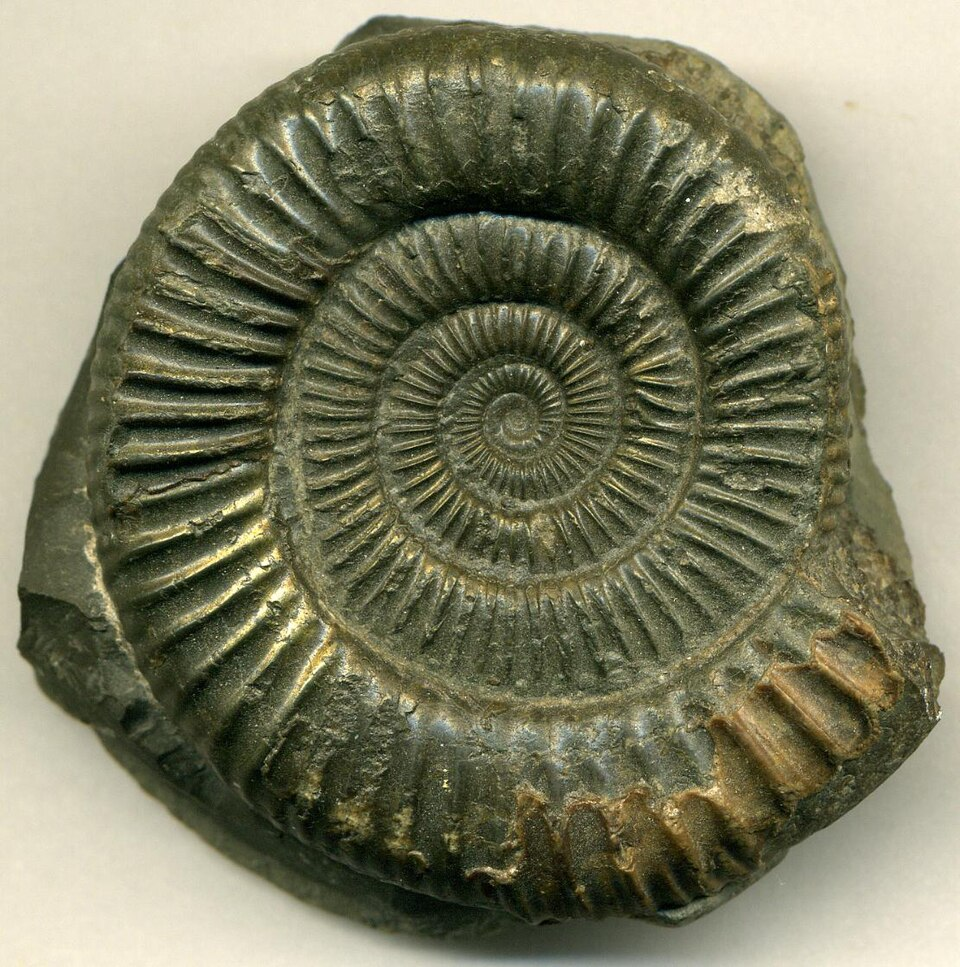
\includegraphics[height=4.6cm]{images/book1/g7-ammonite.jpg}

{\small Un amonites, un animal extinguido con una concha enrollada,
pariente de los calamares y los pulpos, de \qty{5.7}{cm} de diámetro, de
la \omterm{def:g1:landscapes-around-us:water}{costa} de Yorkshire (Inglaterra).}
\end{minipage}\hfill
\begin{minipage}[t]{0.49\linewidth}\centering
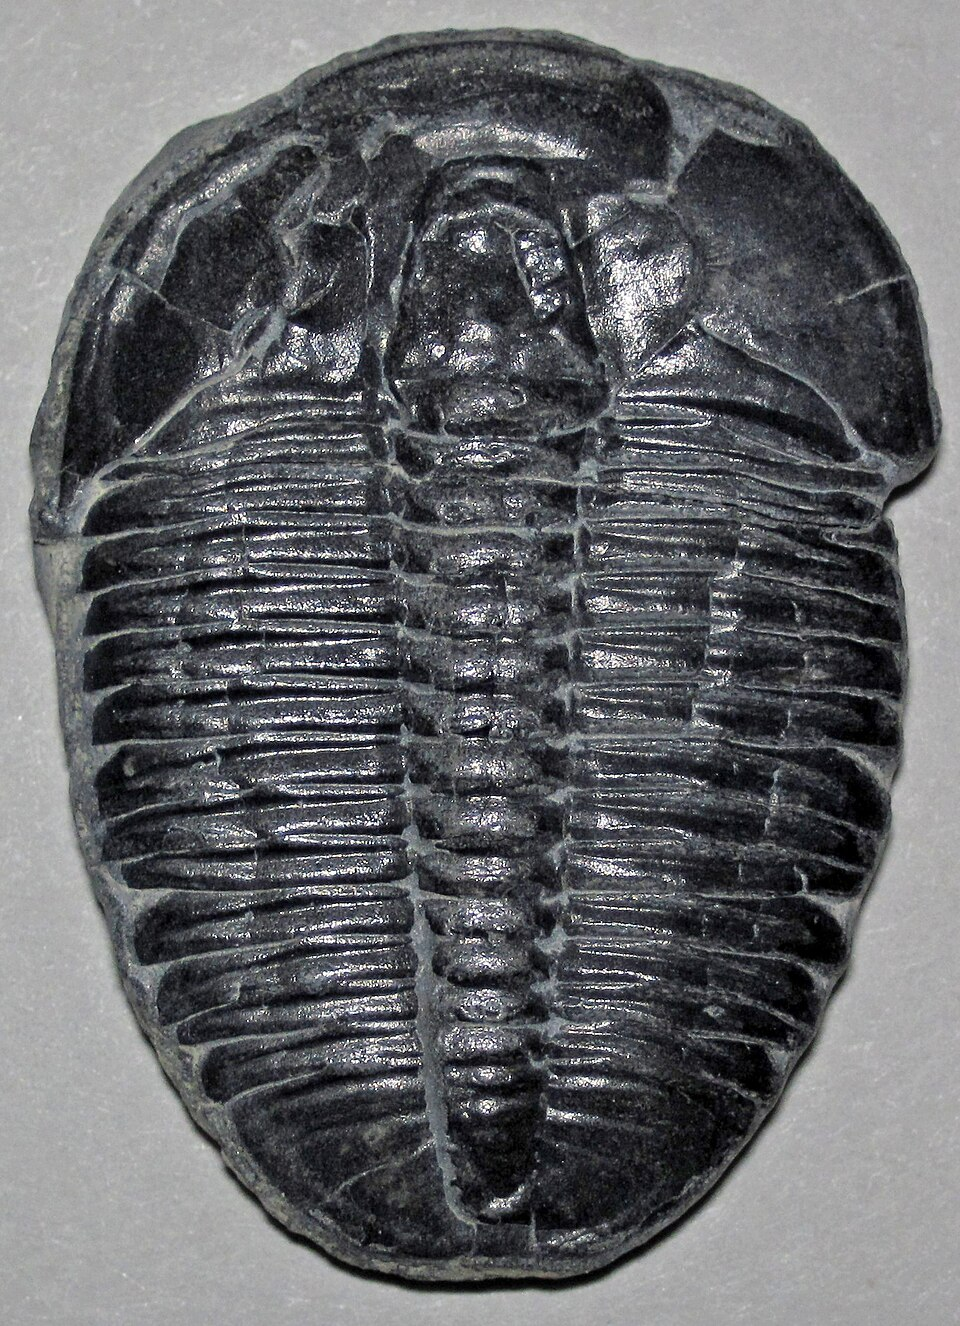
\includegraphics[height=4.6cm]{images/book1/g7-trilobite.jpg}

{\small Un trilobites, un animal marino extinguido cuyo cuerpo tiene tres
lóbulos, de unos \qty{2.6}{cm} de ancho, de Utah (Estados Unidos).}
\end{minipage}\par\medskip

{\small Dos \omterm{def:g7:sediments-and-fossils:fossil}{fósiles} de animales con concha dura. Fotografías: James
St.~John (CC BY 2.0, vía Wikimedia Commons).}
% ledger: commons:ammonite, commons:trilobite, nps:ammonoid, nps:trilobite
\label{fig:g7:sediments-and-fossils:ammonite-trilobite}
\end{omfigure}

A veces la propia concha no dura. Enterrada en la \omterm{def:g3:stones-pebbles-sand:sand}{arena}, el agua que se
filtra entre los granos la disuelve poco a poco, y solo queda un hueco con
la forma de la concha impresa en sus paredes: un \omterm{def:g7:sediments-and-fossils:fossil}{molde}. Si más tarde se
depositan \omterm{def:g6:rocks-and-minerals:mineral}{minerales} en el hueco y lo rellenan, forman una copia de la
concha: un \omterm{def:g7:sediments-and-fossils:fossil}{contramolde}.
% ledger: ucmp:casts-molds

\begin{omfigure}
\begin{tikzpicture}[font=\small, x=1cm, y=1cm,
    clam/.style={line width=0.5pt}]
  \foreach \p/\fillc/\title in {0/{omLithSand!50!white}/{una concha enterrada\\[-2pt]en la arena}, 1/{white}/{la concha se ha disuelto:\\[-2pt]un molde}, 2/{black!40}/{los minerales rellenan el molde:\\[-2pt]un contramolde}} {
    \begin{scope}[xshift=\p*4.9cm]
      \fill[omLithSand] (0,0) rectangle (4.2,2.6);
      \foreach \i in {0,...,40} {
        \pgfmathsetmacro{\gx}{0.1+mod(\i*0.53,4.0)}
        \pgfmathsetmacro{\gy}{0.1+mod(\i*0.37,2.4)}
        \fill[brown!60!black] (\gx,\gy) circle (0.025);
      }
      \fill[\fillc, draw=brown!40!black, clam] (0.9,0.9) arc[start angle=180, end angle=0, x radius=1.2, y radius=0.95] -- cycle;
      \ifnum\p=1
        \foreach \a in {25,45,...,155} \draw[brown!50!black, line width=0.4pt] (2.1,0.9) -- ++(\a:0.93 and 0.75);
      \else
        \foreach \a in {25,45,...,155} \draw[brown!40!black, line width=0.4pt] (2.1,0.9) -- ++(\a:1.05 and 0.85);
      \fi
      \draw[black!70, line width=0.5pt] (0,0) rectangle (4.2,2.6);
      \node[anchor=north, align=center] at (2.1,-0.1) {\title};
    \end{scope}
  }
  \draw[-{Stealth[length=2.5mm]}, line width=1pt] (4.3,1.3) -- (4.8,1.3);
  \draw[-{Stealth[length=2.5mm]}, line width=1pt] (9.2,1.3) -- (9.7,1.3);
\end{tikzpicture}

{\small Un \omterm{def:g7:sediments-and-fossils:fossil}{molde} y un \omterm{def:g7:sediments-and-fossils:fossil}{contramolde} (un dibujo, en corte a través de la
\omterm{def:g3:stones-pebbles-sand:rock}{roca}). El \omterm{def:g7:sediments-and-fossils:fossil}{molde} es el hueco, con las costillas de la concha impresas en su
pared; el \omterm{def:g7:sediments-and-fossils:fossil}{contramolde} es una copia de piedra de la concha, hecha de los
\omterm{def:g6:rocks-and-minerals:mineral}{minerales} que lo rellenaron.}
% ledger: ucmp:casts-molds
\label{fig:g7:sediments-and-fossils:mould-cast}
\end{omfigure}

Los animales también dejan \omterm{def:g7:sediments-and-fossils:fossil}{fósiles} de lo que hicieron. Un animal que
camina sobre el \omterm{def:g3:stones-pebbles-sand:sand}{barro} blando y mojado de la orilla de un \omterm{def:g1:landscapes-around-us:water}{río} o de una
\omterm{def:g1:landscapes-around-us:water}{costa} deja huellas. La mayoría se las lleva la ola o la \omterm{def:g5:water-shapes-the-land:flood}{crecida} siguiente.
Pero si la \omterm{def:g3:stones-pebbles-sand:sand}{arena} las cubre antes de que se borren, la huella se rellena,
más tarde la \omterm{def:g3:stones-pebbles-sand:sand}{arena} se convierte en arenisca, y cuando la \omterm{def:g3:stones-pebbles-sand:rock}{roca} se parte por
esa capa, aparecen la huella y, en la otra cara, su \omterm{def:g7:sediments-and-fossils:fossil}{contramolde}.
% ledger: ucmp:footprints

\begin{omfigure}
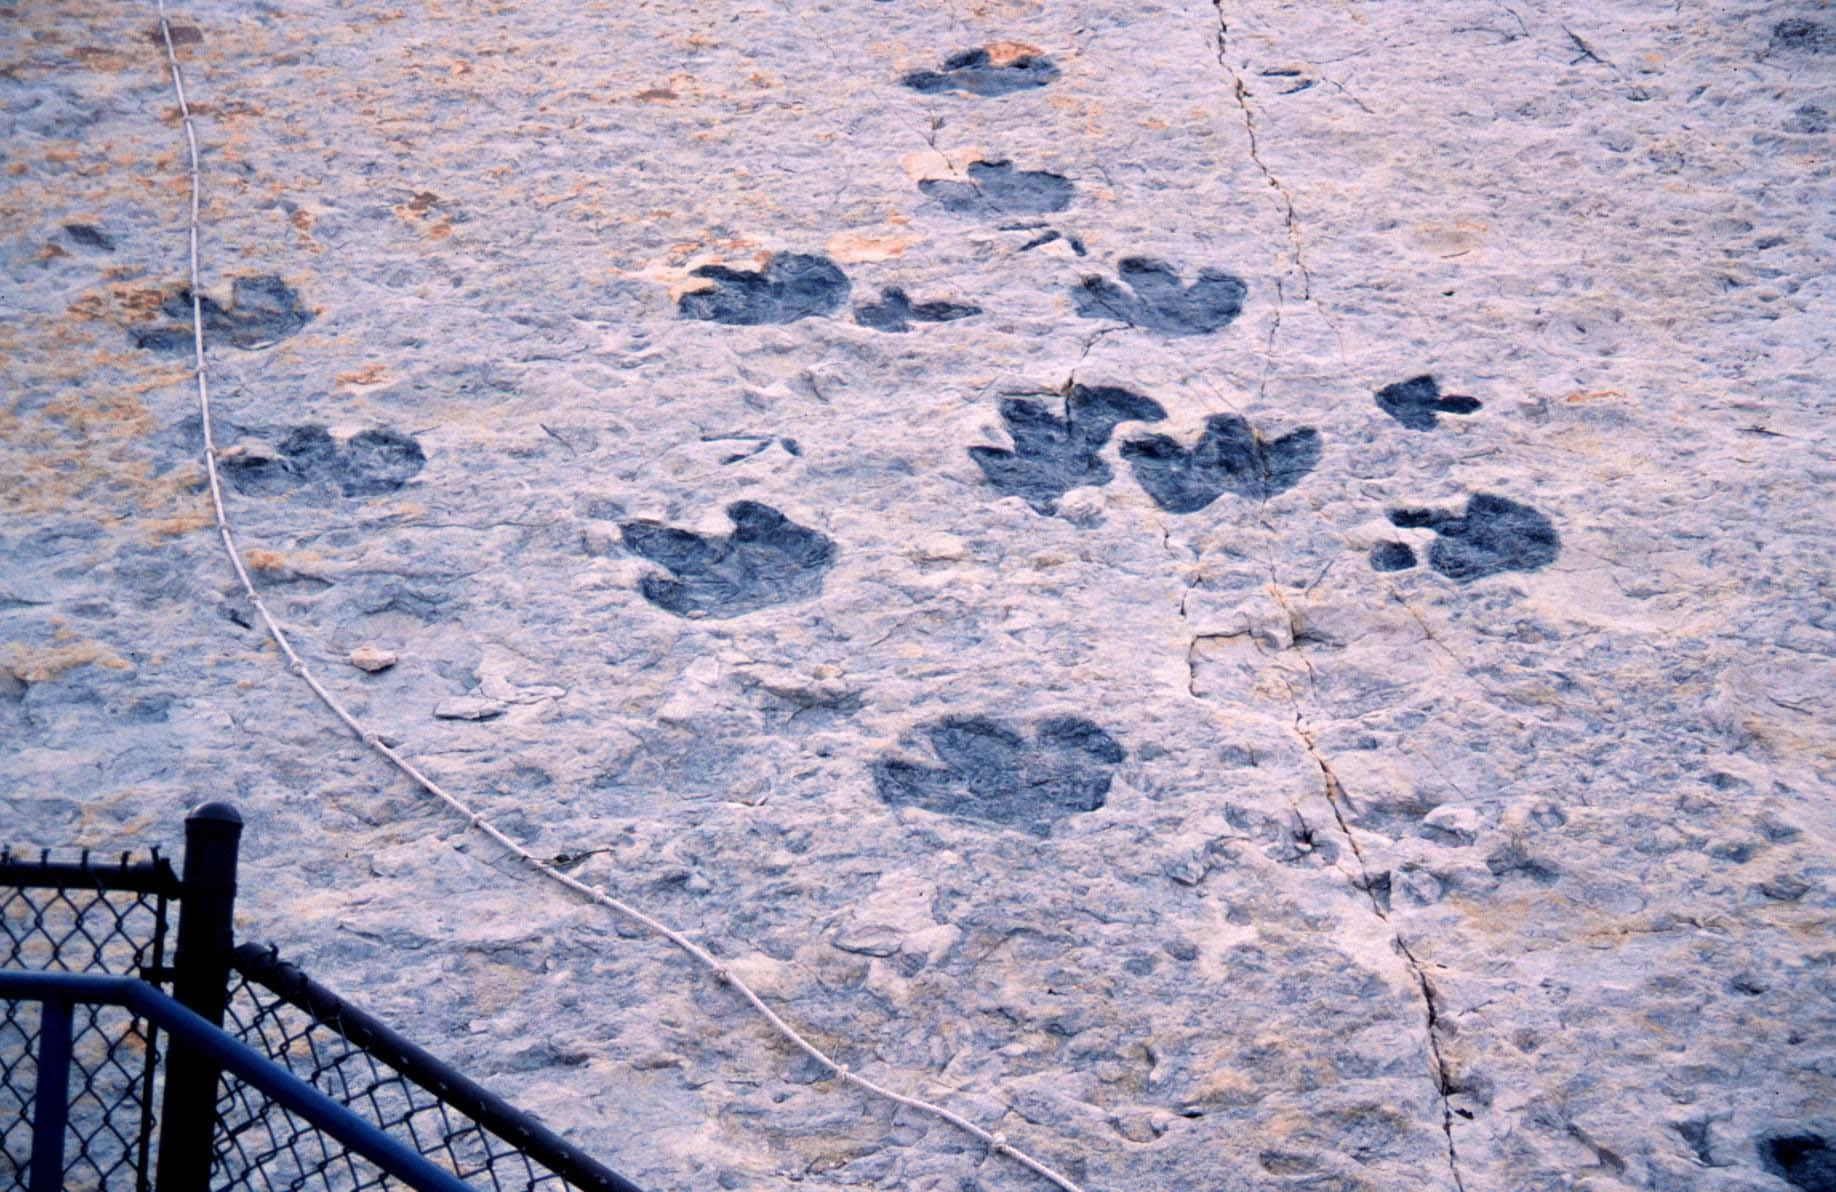
\includegraphics[width=0.62\linewidth]{images/book1/g7-dinosaur-tracks.jpg}

{\small Huellas de dinosaurios en Dinosaur Ridge, cerca de Morrison,
Colorado (Estados Unidos): decenas de rastros dejados en un suelo blando,
hoy una superficie de \omterm{def:g3:stones-pebbles-sand:rock}{roca} inclinada. La mayoría las dejaron dinosaurios
herbívoros, y unas pocas, carnívoros de dedos finos. Fotografía: Dexter
Perkins (CC0, vía Wikimedia Commons).}
% ledger: commons:dino-tracks
\label{fig:g7:sediments-and-fossils:tracks}
\end{omfigure}

La biología usa los \omterm{def:g7:sediments-and-fossils:fossil}{fósiles} para seguir la larga historia de los seres
vivos. En este libro, los \omterm{def:g7:sediments-and-fossils:fossil}{fósiles} son pistas de otra clase: nos dicen cómo
era el lugar cuando el animal vivía allí.

\section{Capas y fósiles, un registro del pasado}

Cada capa guarda las marcas del lugar donde se depositó. Los arrecifes de
coral crecen hoy en \omterm{def:g2:water-on-earth:ocean}{mares} cálidos, transparentes y poco profundos; las
rizaduras se forman sobre la \omterm{def:g3:stones-pebbles-sand:sand}{arena} en aguas poco profundas, en la orilla
de un \omterm{def:g1:landscapes-around-us:water}{lago}, de un \omterm{def:g1:landscapes-around-us:water}{río} o de un \omterm{def:g2:water-on-earth:ocean}{mar}; el carbón se formó a partir de las
plantas de antiguos bosques y marismas; los braquiópodos, los crinoideos y
los trilobites solo vivían en el \omterm{def:g2:water-on-earth:ocean}{mar}. Cuando se encuentran las mismas
pistas en una capa antigua, es probable que el lugar fuera así cuando se
formó la capa.
% ledger: noaa:coral-where, nps:ripple-marks, nps:ripples-shallow, usgs:coal-origin, nps:trilobite

\begin{center}
\small
\begin{tabular}{|p{0.36\linewidth}|p{0.52\linewidth}|}
\hline
\textbf{pista en la capa} & \textbf{el lugar cuando se formó la capa} \\
\hline
corales & un \omterm{def:g2:water-on-earth:ocean}{mar} cálido, poco profundo y transparente \\
\hline
conchas de animales marinos (braquiópodos, crinoideos, trilobites) & un \omterm{def:g2:water-on-earth:ocean}{mar} \\
\hline
rizaduras en la superficie de una capa & aguas poco profundas, en la orilla de un \omterm{def:g1:landscapes-around-us:water}{lago}, de un \omterm{def:g1:landscapes-around-us:water}{río} o de un \omterm{def:g2:water-on-earth:ocean}{mar} \\
\hline
huellas de pisadas & \omterm{def:g3:stones-pebbles-sand:sand}{barro} o \omterm{def:g3:stones-pebbles-sand:sand}{arena} blandos y mojados, a menudo en una \omterm{def:g1:landscapes-around-us:water}{costa} o en la orilla de un \omterm{def:g1:landscapes-around-us:water}{río} \\
\hline
carbón & un bosque pantanoso o una marisma \\
\hline
hojas y alas de libélula & tierra firme, con plantas \\
\hline
\end{tabular}
\end{center}
% ledger: noaa:coral-where, nps:grca-fossils, nps:trilobite, nps:ripple-marks, nps:ripples-shallow, ucmp:footprints, usgs:coal-origin

\begin{method}[Leer una capa]\label{met:g7:sediments-and-fossils:reading}
\begin{enumerate}
  \item Mira los granos: los granos gruesos se depositan donde el agua se
        mueve deprisa, y el \omterm{def:g3:stones-pebbles-sand:sand}{barro} fino solo donde está tranquila.
  \item Busca \omterm{def:g7:sediments-and-fossils:fossil}{fósiles} y marcas (corales, conchas, huellas, rizaduras,
        restos de plantas, carbón) y usa la tabla de arriba.
  \item Junta las pistas en una sola imagen del lugar: tierra firme o \omterm{def:g2:water-on-earth:ocean}{mar},
        aguas someras o profundas, agua tranquila o en movimiento.
\end{enumerate}
\end{method}

\begin{omfigure}
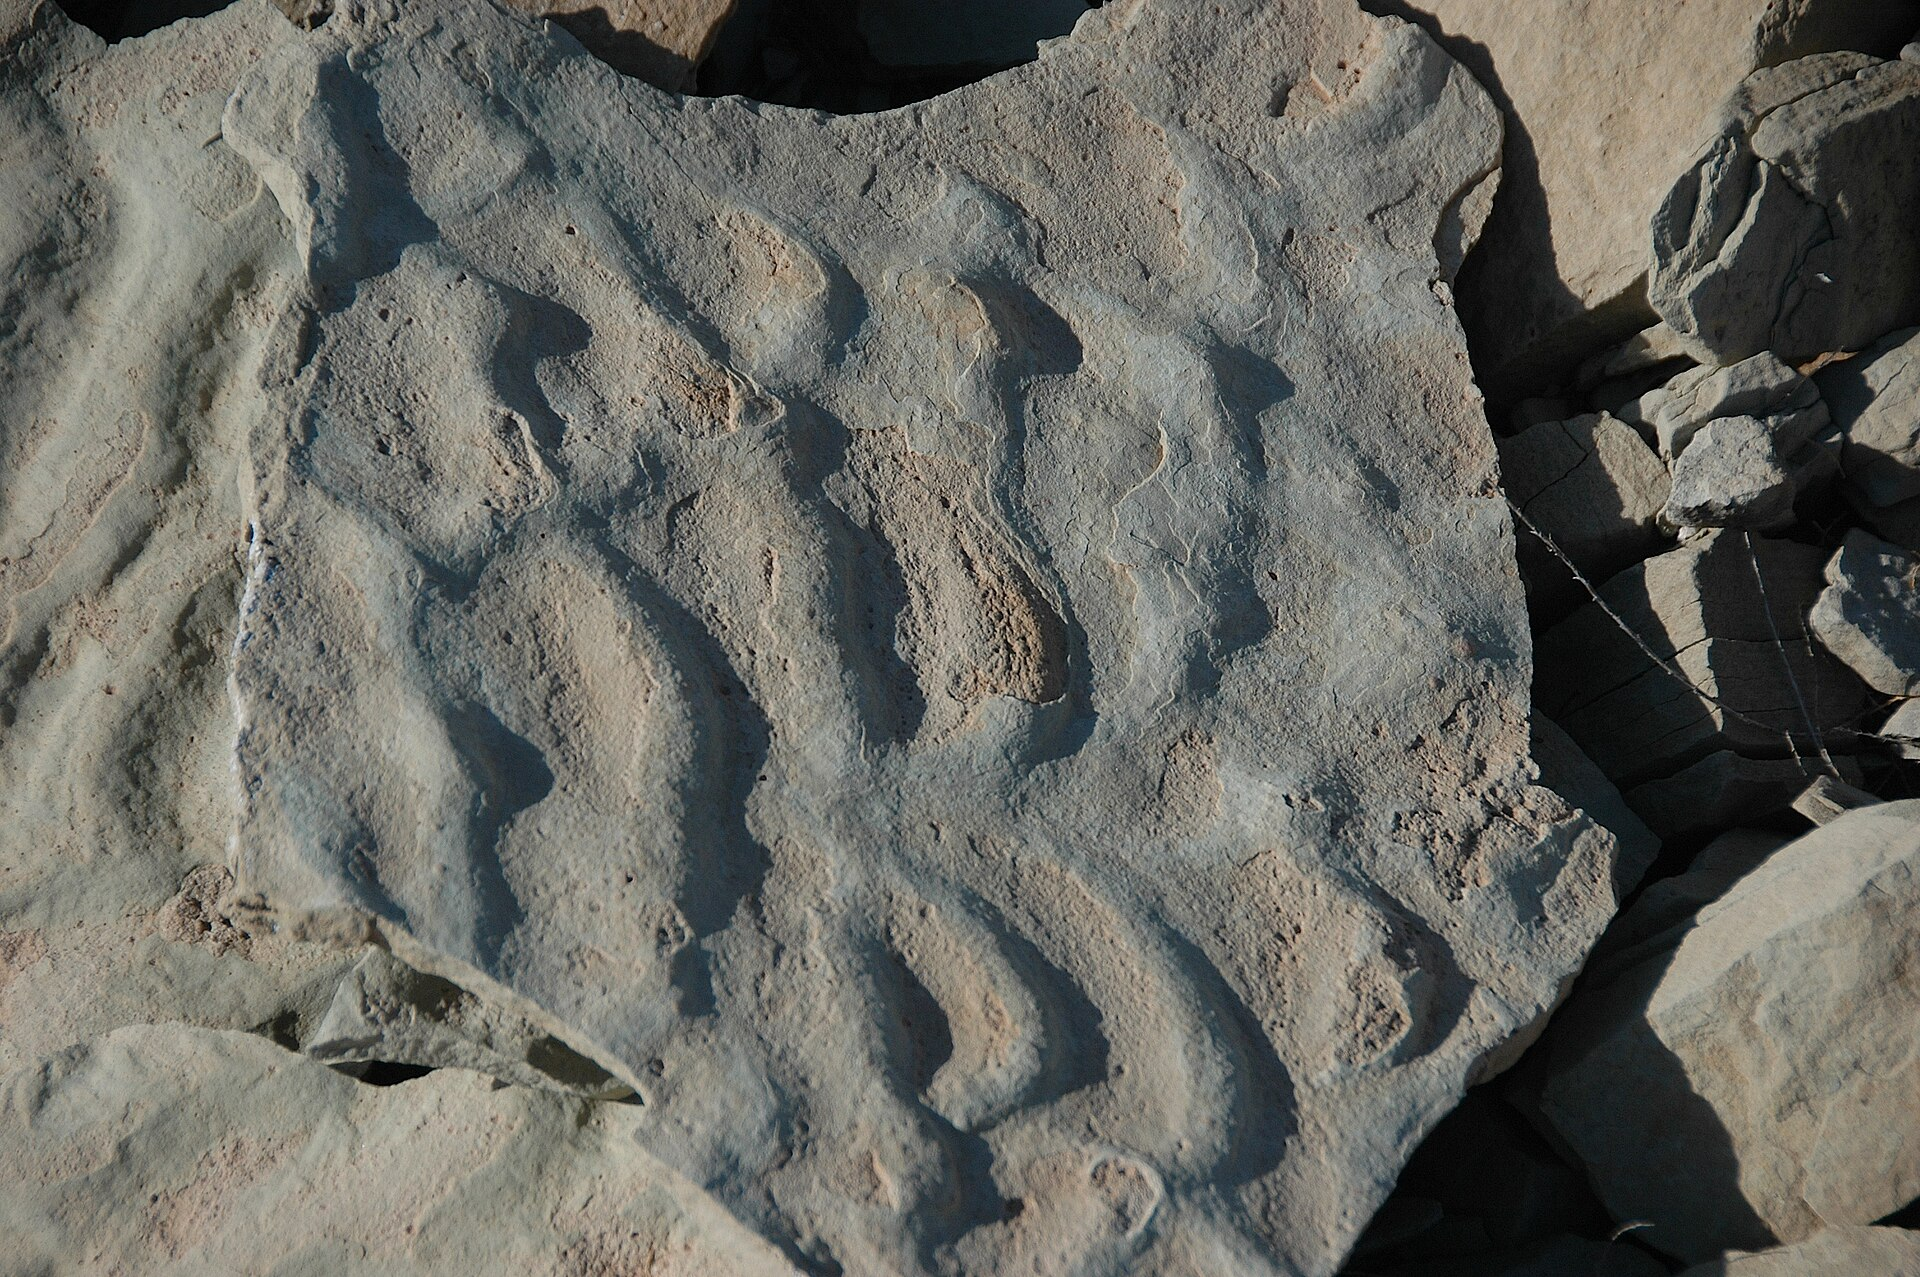
\includegraphics[width=0.56\linewidth]{images/book1/g7-ripple-marks.jpg}

{\small Rizaduras sobre una losa de arenisca del Parque Nacional Capitol
Reef, en Utah (Estados Unidos): el agua en movimiento ondulaba en otro
tiempo esta \omterm{def:g3:stones-pebbles-sand:sand}{arena}, como la \omterm{def:g3:stones-pebbles-sand:sand}{arena} de una playa o del lecho de un arroyo hoy.
Fotografía: James St.~John (CC BY 2.0, vía Wikimedia Commons).}
% ledger: commons:ripples, nps:ripple-marks
\label{fig:g7:sediments-and-fossils:ripples}
\end{omfigure}

\begin{example}[La parte alta del Gran Cañón]\label{ex:g7:sediments-and-fossils:kaibab}
La caliza de Kaibab, la capa más alta del Gran Cañón, está llena de
conchas de braquiópodos y de trozos de tallo de crinoideos, dos animales
marinos. Se formó en el fondo de un \omterm{def:g2:water-on-earth:ocean}{mar}. Hoy esa misma capa está hasta a
unos \qty{2700}{m} (\num{9000}~pies) sobre el \omterm{def:g4:world-physical-map:altitude}{nivel del mar}: desde que se
formó, toda la región se ha elevado.
% ledger: nps:grca-fossils, nps:grca-kaibab
\end{example}

Un montón de capas se puede dibujar como una \emph{columna}: las capas
apiladas en el orden en que se formaron, con su espesor a escala y sus
pistas anotadas al lado. Abajo está la columna de las Colinas de Varden, la
región inventada de los ejercicios de esta serie.

\begin{omfigure}
\begin{tikzpicture}
  \begin{axis}[width=4.2cm, height=9.2cm, scale only axis=false, xmin=0, xmax=1, ymin=-60, ymax=485,
      axis x line=none, axis y line*=left, ytick={0,100,200,300,400},
      ylabel={metros sobre la base de la arenisca}, label style={font=\footnotesize},
      tick label style={font=\scriptsize}, clip=false]
    \addplot[lith schist, draw=black!70, line width=0.3pt] table {figdata/out/grade-7-varden_column-unit-older.dat};
    \addplot[lith sandstone, draw=black!70, line width=0.3pt] table {figdata/out/grade-7-varden_column-unit-sandstone.dat};
    \addplot[lith limestone, draw=black!70, line width=0.3pt] table {figdata/out/grade-7-varden_column-unit-limestone.dat};
    \addplot[lith shale, draw=black!70, line width=0.3pt] table {figdata/out/grade-7-varden_column-unit-shale.dat};
    \addplot[om lith={white}{om limestone}, draw=black!70, line width=0.3pt] table {figdata/out/grade-7-varden_column-unit-chalk.dat};
    \node[anchor=west, align=left, font=\footnotesize] at (axis cs:1.12,450) {\textbf{creta}: su techo se ha\\desgastado (solo se dibuja su base)};
    \node[anchor=west, align=left, font=\footnotesize] at (axis cs:1.12,350) {\textbf{lutita}, \qty{100}{m}: granos muy finos;\\amonites};
    \node[anchor=west, align=left, font=\footnotesize] at (axis cs:1.12,210) {\textbf{caliza}, \qty{180}{m}:\\corales y conchas};
    \node[anchor=west, align=left, font=\footnotesize] at (axis cs:1.12,60) {\textbf{arenisca}, \qty{120}{m}:\\rizaduras, huellas};
    \node[anchor=west, align=left, font=\footnotesize] at (axis cs:1.12,-30) {rocas más antiguas (esquisto y granito),\\desgastadas hasta quedar planas antes de la arenisca};
  \end{axis}
\end{tikzpicture}

\medskip
{\small La columna de las Colinas de Varden, la región inventada de esta
serie: las capas en el orden en que se formaron, la primera abajo, con sus
espesores a escala. Los \omterm{def:g7:sediments-and-fossils:fossil}{fósiles} y las marcas anotados al lado son datos de
ejercicio.}
% ledger: (invented region: figdata/shared/region.py, drawn by figdata/grade-7/varden_column.py)
\label{fig:g7:sediments-and-fossils:column}
\end{omfigure}

\begin{omfigure}
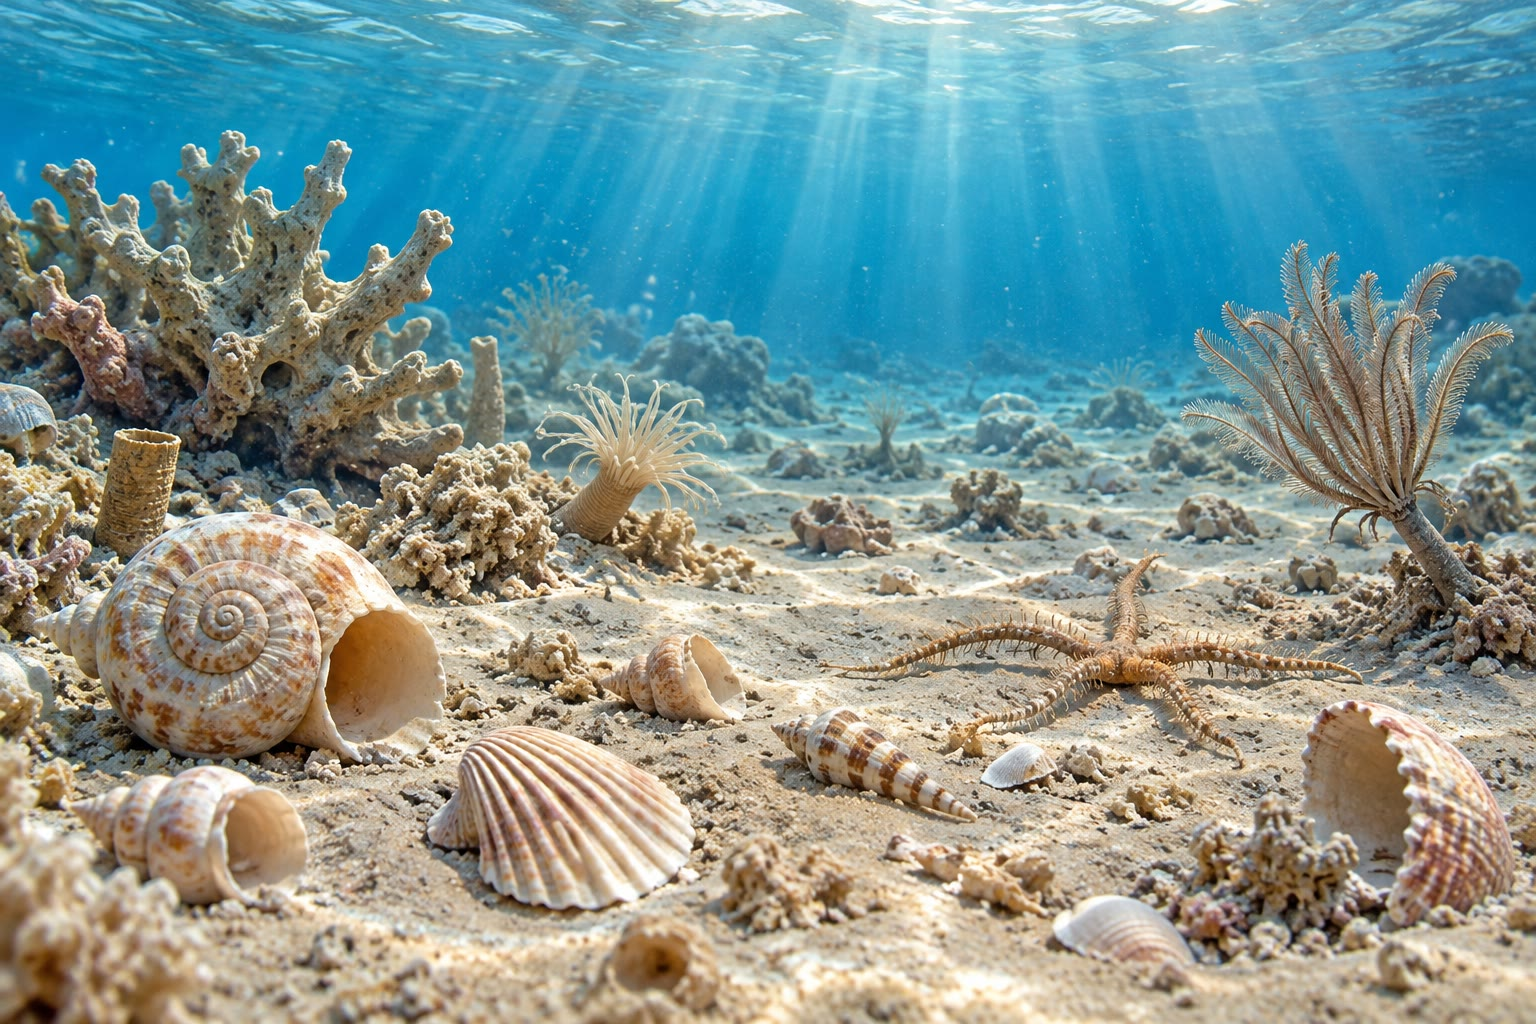
\includegraphics[width=0.6\linewidth]{images/book1/ai/g7-shallow-sea.jpg}

{\small El fondo de un \omterm{def:g2:water-on-earth:ocean}{mar} cálido y poco profundo de hace mucho tiempo, tal
como podía ser mientras las conchas y los trozos de coral se depositaban
para formar una futura caliza (ilustración generada por IA de una escena
genérica).}
\label{fig:g7:sediments-and-fossils:shallow-sea}
\end{omfigure}

\begin{remark}[Mira, fotografía y déjalo]\label{rem:g7:sediments-and-fossils:leave}
En muchos lugares protegidos está prohibido llevarse un \omterm{def:g7:sediments-and-fossils:fossil}{fósil}: en el Gran
Cañón, por ejemplo, la ley prohíbe desenterrar, mover o llevarse cualquier
\omterm{def:g7:sediments-and-fossils:fossil}{fósil}. Quien encuentra uno lo fotografía o lo dibuja, lo deja donde está
para que otros lo vean y los científicos lo estudien, y avisa a un guarda
del parque.
\end{remark}
% ledger: nps:grca-fossils

\begin{inthefield}[Sedimentos que se depositan hoy]
En una playa, en la orilla de un \omterm{def:g1:landscapes-around-us:water}{lago} o de un arroyo, con un adulto, mira
la \omterm{def:g3:stones-pebbles-sand:sand}{arena} bajo el agua poco profunda: el agua en movimiento le da forma de
ondulaciones, como las que conserva la arenisca antigua. Deja una huella
en la \omterm{def:g3:stones-pebbles-sand:sand}{arena} mojada junto al borde del agua y observa qué le hacen las olas
siguientes. Después de un día de \omterm{def:g4:clouds-rain-snow:precipitation}{lluvia}, mira un charco que se haya
secado: una fina película de \omterm{def:g3:stones-pebbles-sand:sand}{barro} suele cubrir la \omterm{def:g3:stones-pebbles-sand:sand}{arena} del fondo ---
los granos más finos, que se depositaron los últimos, cuando el agua
estaba quieta. Dibuja lo que veas, y anota dónde y cuándo.
\end{inthefield}
% ledger: nps:ripple-marks, ucmp:footprints, usgs:strata

\section{Ejercicios}

\begin{exercise}[$\star$]\label{exo:g7:sediments-and-fossils:1}
Une cada palabra con su significado: \omterm{def:g7:sediments-and-fossils:sediment}{sedimento}; \omterm{def:g7:sediments-and-fossils:layer}{estrato}; \omterm{def:g7:sediments-and-fossils:fossil}{fósil}; \omterm{def:g7:sediments-and-fossils:fossil}{molde};
\omterm{def:g7:sediments-and-fossils:fossil}{contramolde}; \omterm{def:g7:sediments-and-fossils:fossil}{icnofósil}. (a) Un hueco que queda en una \omterm{def:g3:stones-pebbles-sand:rock}{roca} donde se ha
disuelto una concha. (b) Una huella o una madriguera conservada en una
\omterm{def:g3:stones-pebbles-sand:rock}{roca}. (c) Material suelto depositado por el agua, el viento o el hielo.
(d) Una copia de piedra que se forma cuando un hueco se rellena de
\omterm{def:g6:rocks-and-minerals:mineral}{minerales}. (e) Una lámina de \omterm{def:g7:sediments-and-fossils:sediment}{sedimento} depositada de una sola vez. (f) El
resto o la huella de un ser vivo de hace mucho tiempo, conservado en una
\omterm{def:g3:stones-pebbles-sand:rock}{roca}.
\end{exercise}

\begin{exercise}[$\star$]\label{exo:g7:sediments-and-fossils:2}
Ordena estas etapas para contar cómo una concha se convierte en un \omterm{def:g7:sediments-and-fossils:fossil}{fósil}
que aparece en la superficie: (a) la \omterm{def:g5:water-shapes-the-land:erosion}{erosión} desgasta las capas de encima;
(b) el animal muere en el fondo del \omterm{def:g2:water-on-earth:ocean}{mar}; (c) se acumulan capas nuevas y la
concha se convierte en piedra; (d) el \omterm{def:g3:stones-pebbles-sand:sand}{barro} cubre la concha deprisa.
\end{exercise}

\begin{exercise}[$\star$]\label{exo:g7:sediments-and-fossils:3}
Usa la tabla de las pistas. ¿Dónde se formó cada capa? (a) Una caliza
llena de corales. (b) Una arenisca cuya superficie muestra rizaduras.
(c) Una capa oscura de carbón. (d) Una lutita con huellas de hojas y el
ala de una libélula.
\end{exercise}

\begin{exercise}[$\star$]\label{exo:g7:sediments-and-fossils:4}
¿Verdadero o falso? Corrige las falsas. (a) Todo animal que muere se
convierte algún día en \omterm{def:g7:sediments-and-fossils:fossil}{fósil}. (b) Una huella de pisada puede ser un \omterm{def:g7:sediments-and-fossils:fossil}{fósil}.
(c) Cuando el agua cargada de \omterm{def:g3:stones-pebbles-sand:sand}{barro} frena, el \omterm{def:g3:stones-pebbles-sand:sand}{barro} fino se deposita
primero. (d) Los \omterm{def:g7:sediments-and-fossils:sediment}{sedimentos} se depositan en capas horizontales.
\end{exercise}

\begin{exercise}[$\star\star$]\label{exo:g7:sediments-and-fossils:5}
Usa la columna de las Colinas de Varden. (a) Da el espesor de la arenisca,
de la caliza y de la lutita. (b) ¿Cuál es su espesor total? (c) ¿Qué
porcentaje de ese total es caliza? Redondea al número entero más cercano.
(d) ¿Por qué la columna no da ningún espesor para la creta?
\end{exercise}

\begin{exercise}[$\star\star$]\label{exo:g7:sediments-and-fossils:6}
Una alumna agita un tarro de agua con \omterm{def:g3:stones-pebbles-sand:pebble}{grava}, \omterm{def:g3:stones-pebbles-sand:sand}{arena} y \omterm{def:g3:stones-pebbles-sand:sand}{barro}, y deja que se
deposite. (a) Dibuja el tarro al día siguiente y rotula las capas. (b) ¿Por
qué el agua sigue turbia al cabo de una hora? (c) Vuelve a añadir \omterm{def:g3:stones-pebbles-sand:sand}{arena} y
\omterm{def:g3:stones-pebbles-sand:sand}{barro} y deja que se deposite. ¿Qué ve ahora en el fondo? (d) ¿Qué capa del
tarro se formó primero?
\end{exercise}

\begin{exercise}[$\star\star$]\label{exo:g7:sediments-and-fossils:7}
¿Cuál de estos restos tiene más posibilidades de convertirse en \omterm{def:g7:sediments-and-fossils:fossil}{fósil}, y
cuál menos? Explícalo. (a) Una medusa arrastrada hasta una \omterm{def:g1:landscapes-around-us:water}{costa} rocosa.
(b) Una concha de caracol enterrada en el \omterm{def:g3:stones-pebbles-sand:sand}{barro} de un \omterm{def:g1:landscapes-around-us:water}{lago} tranquilo.
(c) Un hueso que lleva años en una \omterm{def:g1:landscapes-around-us:landform}{llanura} seca. (d) Una concha de almeja
cubierta de \omterm{def:g3:stones-pebbles-sand:sand}{arena} durante una \omterm{def:g5:water-shapes-the-land:flood}{crecida} de un \omterm{def:g1:landscapes-around-us:water}{río}.
\end{exercise}

\begin{exercise}[$\star\star$]\label{exo:g7:sediments-and-fossils:8}
Una concha queda enterrada en una \omterm{def:g3:stones-pebbles-sand:sand}{arena} que se convierte en arenisca. El
agua que se filtra a través de la \omterm{def:g3:stones-pebbles-sand:rock}{roca} disuelve la concha por completo.
(a) ¿Qué queda en la \omterm{def:g3:stones-pebbles-sand:rock}{roca}? (b) Más tarde, unos \omterm{def:g6:rocks-and-minerals:mineral}{minerales} rellenan ese
hueco. ¿Qué se forma? (c) ¿Sigue estando allí la propia concha? (d) ¿Por
qué se encuentran \omterm{def:g7:sediments-and-fossils:fossil}{moldes} y \omterm{def:g7:sediments-and-fossils:fossil}{contramoldes} más a menudo en la arenisca que en
la lutita? (Piensa en lo fácilmente que pasa el agua entre los granos.)
\end{exercise}

\begin{exercise}[$\star\star$]\label{exo:g7:sediments-and-fossils:9}
El Gran Cañón tiene de media \qty{1.6}{km} de profundidad. (a) Escribe esta
profundidad en metros. (b) Supón que las paredes del cañón estuvieran
hechas de capas de \qty{80}{m} de espesor cada una: ¿cuántas capas cabrían
desde el borde hasta el fondo? (c) ¿Qué porcentaje de la profundidad es
una capa de \qty{160}{m}?
\end{exercise}

\begin{exercise}[$\star\star$]\label{exo:g7:sediments-and-fossils:10}
En una arenisca se encuentran huellas de dinosaurios. (a) ¿Caminaban los
dinosaurios sobre \omterm{def:g3:stones-pebbles-sand:rock}{roca} dura? Explícalo. (b) ¿Por qué desaparecen la
mayoría de las huellas que se dejan en una orilla embarrada? (c) ¿Qué tuvo
que ocurrir poco después de que pasaran los dinosaurios para que se
conservaran las huellas? (d) ¿Es una huella un \omterm{def:g7:sediments-and-fossils:fossil}{fósil} corporal o un
\omterm{def:g7:sediments-and-fossils:fossil}{icnofósil}?
\end{exercise}

\begin{exercise}[$\star\star\star$]\label{exo:g7:sediments-and-fossils:11}
En un \omterm{def:g1:landscapes-around-us:water}{lago}, cada \omterm{def:g5:water-shapes-the-land:flood}{crecida} deja una capa de \omterm{def:g3:stones-pebbles-sand:sand}{arena} de unos \qty{2}{cm} de
espesor, y las semanas tranquilas que la siguen, una capa de \omterm{def:g3:stones-pebbles-sand:sand}{barro} de unos
\qty{5}{mm} (datos de ejercicio). (a) ¿Qué espesor tiene, en milímetros,
un par de capas? (b) Un testigo extraído del fondo del \omterm{def:g1:landscapes-around-us:water}{lago} mide \qty{1}{m}
de largo y solo está formado por pares como esos. ¿Cuántas \omterm{def:g5:water-shapes-the-land:flood}{crecidas}
registra? (c) Cerca de la \omterm{def:g5:water-shapes-the-land:source-mouth}{desembocadura} del \omterm{def:g1:landscapes-around-us:water}{río}, las capas de \omterm{def:g3:stones-pebbles-sand:sand}{arena} son
más gruesas, y lejos, más finas. Explica por qué. (d) ¿Por qué hay más
\omterm{def:g3:stones-pebbles-sand:sand}{barro} que \omterm{def:g3:stones-pebbles-sand:sand}{arena} lejos de la \omterm{def:g5:water-shapes-the-land:source-mouth}{desembocadura}?
\end{exercise}

\begin{exercise}[$\star\star\star$]\label{exo:g7:sediments-and-fossils:12}
Los \omterm{def:g7:sediments-and-fossils:fossil}{fósiles} que se encuentran en las \omterm{def:g3:stones-pebbles-sand:rock}{rocas} son sobre todo conchas y restos
diminutos; los \omterm{def:g7:sediments-and-fossils:fossil}{fósiles} de animales blandos son raros, y los dinosaurios
solo son una parte muy pequeña de todos los \omterm{def:g7:sediments-and-fossils:fossil}{fósiles}. (a) Explica por qué
las conchas son tan frecuentes. (b) Explica por qué los animales blandos
son raros. (c) Una científica quiere conocer todos los animales que
vivían en un \omterm{def:g2:water-on-earth:ocean}{mar} antiguo. ¿Pueden los \omterm{def:g7:sediments-and-fossils:fossil}{fósiles} darle la lista completa?
Explícalo.
\end{exercise}

\section{Problema: la columna de las Colinas de Varden}

\begin{problem}[{Problema de fin de semana --- se leen una a una las capas
de las Colinas de Varden, sus fósiles dicen dónde se formaron y se calcula
el tiempo necesario para acumular la caliza}]
\label{pb:g7:sediments-and-fossils:1}
% ledger: (invented region: figdata/shared/region.py; rates are exercise data, figdata/grade-7/varden_column.py part rates)
Usa la columna de las Colinas de Varden de este capítulo. Su arenisca
muestra rizaduras y huellas; su caliza contiene corales y conchas; su
lutita está hecha de granos muy finos, con amonites; la creta de lo alto
se ha desgastado en parte.

\medskip
\noindent\textbf{Parte I --- Leer las capas.}\par\nopagebreak
\begin{enumerate}[beginpenalty=10000]
  \item Enumera las cuatro capas, de la primera que se depositó a la
        última.
  \item Da el espesor de la arenisca, de la caliza y de la lutita, y su
        total.
  \item ¿Qué porcentaje de ese total es caliza?
  \item ¿Por qué nadie puede decir qué espesor tenía la creta cuando se
        formó?
\end{enumerate}

\medskip
\noindent\textbf{Parte II --- Sus fósiles.}\par\nopagebreak
\begin{enumerate}[resume, beginpenalty=10000]
  \item ¿Dónde se formó la arenisca? Da dos pistas.
  \item ¿Dónde se formó la caliza? Da la pista.
  \item La lutita está hecha de granos muy finos. ¿Estaba el agua tranquila
        o en movimiento cuando se depositó? Explícalo.
  \item Cuenta la historia del lugar en tres frases, de la arenisca a la
        lutita.
\end{enumerate}

\medskip
\noindent\textbf{Parte III --- Cuánto tiempo llevó.}\par\nopagebreak
\begin{enumerate}[resume, beginpenalty=10000]
  \item Escribe el espesor de la caliza en centímetros.
  \item Supón que la arenisca se acumuló a razón de \qty{1}{cm} cada
        20 años. ¿Cuántos años tardaron en formarse sus \qty{120}{m}?
  \item Supón que la caliza se acumuló a razón de \qty{1}{cm} cada
        100 años. ¿Cuántos años tardó en formarse \qty{1}{m} de caliza?
  \item ¿Cuántos años tardaron en formarse los \qty{180}{m} de caliza?
        ¿Cuántas veces más que la arenisca es eso?
\end{enumerate}
\end{problem}
